%%%%%%%%%%%%%%%%%%%%%%%%%%%%%%%%%%%%%%%%%%%%%%%%%%%%%%%%%%%%%%%%%%%%%%%%%%%%%%%%%%%%%%%%%
%
% Presentation: Privacy-Preserving Multi-Agent Intelligent Chatbot for PCOS Diagnosis
% Built on the DEE@ISEP Beamer template by Vitor M. R. Cunha (CC BY 4.0);
% ISEP-specific branding is overridden in preamble.tex.
%
% Build:  tectonic main.tex     (or: latexmk -pdf main.tex)
%
%%%%%%%%%%%%%%%%%%%%%%%%%%%%%%%%%% CLASS SETTINGS %%%%%%%%%%%%%%%%%%%%%%%%%%%%%%%%%%%%%%

\documentclass[
aspectratio=169,	% Comment for 4:3 aspect ratio
english,			% Document language
%handout			% Uncomment to make the PDF WITHOUT overlays
]{DEEclassP}

% Use the 'preamble.tex' file (root folder) do add packages and macros. Keep your main.tex file clean.
%%%%%%%%%%%%%%%%%%%%%%%%%%%%%%%%%%%%%%%%%%%%%%%%%%%%%%%%%% packages
\usepackage{amsmath}		% the main package in the AMS-LATEX distribution
\usepackage{amsfonts}		% extended set of fonts for use in mathematics
\usepackage{amssymb}		% adds new symbols to be used in math mode
\usepackage{mathrsfs}		% math fonts, e.g., Laplace
\usepackage{float}			% provides the H float modifier option
\usepackage{multirow}		% tables \multirow command
\usepackage{subcaption}		% enables subfigures
\usepackage{siunitx}
\usepackage{textcomp}
\usepackage{gensymb}		% typesetting of units
\usepackage{verbatim}		% new verbatim environment, \begin{comment}...\end{comment}, \verbatiminput
%add extra packages if needed here

%%%%%%%%%%%%%%%%%%%%%%%%%%%%%%%%%%%%%%%%%%%%%%%%%%%%%%%%%% settings

% Architecture diagram is shared with the project page
\graphicspath{{./figures/}{./theme/}{../diagram/}}

% Accent colour, matching the project page
\definecolor{PCOSrose}{RGB}{190,18,60}
\setbeamercolor{alerted text}{fg=PCOSrose}

%%%%%%%%%%%%%%%%%%%%%%%%%%%%%%%%%%%%%%%%%%%%%%%%%%%%%%%%%% template overrides
% The DEE@ISEP class adds ISEP logos, a degree name and a student number.
% None apply to this paper, so the title page, frame title and footline are
% redefined here without them. DEEclassP.cls itself is left unchanged.

\makeatletter

% Frame title without the ISEP logo
\setbeamertemplate{frametitle}{%
  \nointerlineskip
  \begin{beamercolorbox}[wd=\paperwidth,leftskip=.3cm,rightskip=.3cm plus1fil,vmode]{frametitle}
    \vskip.6ex
    \usebeamerfont{frametitle}\strut\insertframetitle\strut\par
    \ifx\insertframesubtitle\@empty\else
      {\usebeamerfont{framesubtitle}\usebeamercolor[fg]{framesubtitle}\insertframesubtitle\strut\par}%
    \fi
    \vskip.4ex
  \end{beamercolorbox}%
}

% Title page: title, authors, affiliations, date
\setbeamertemplate{title page}{%
  \vbox{}
  \vfill
  \begingroup
    \centering
    \begin{beamercolorbox}[sep=8pt,center]{title}
      \usebeamerfont{title}\inserttitle\par
    \end{beamercolorbox}
    \vskip1.2em
    {\usebeamerfont{author}\insertauthor\par}
    \vskip0.8em
    {\usebeamerfont{institute}\insertinstitute\par}
    \vskip1em
    {\usebeamerfont{date}\insertdate\par}
  \endgroup
  \vfill
}

% Footline: short authors | short title | date | frame number
\setbeamertemplate{footline}{%
  \leavevmode%
  \hbox{%
  \begin{beamercolorbox}[wd=.3\paperwidth,ht=2.25ex,dp=1ex,center]{author in head/foot}%
    \usebeamerfont{author in head/foot}\insertshortauthor
  \end{beamercolorbox}%
  \begin{beamercolorbox}[wd=.45\paperwidth,ht=2.25ex,dp=1ex,center]{title in head/foot}%
    \usebeamerfont{title in head/foot}\insertshorttitle
  \end{beamercolorbox}%
  \begin{beamercolorbox}[wd=.15\paperwidth,ht=2.25ex,dp=1ex,center]{date in head/foot}%
    \usebeamerfont{date in head/foot}\insertshortdate
  \end{beamercolorbox}%
  \begin{beamercolorbox}[wd=.1\paperwidth,ht=2.25ex,dp=1ex,right]{date in head/foot}%
    \insertframenumber{} / \inserttotalframenumber\hspace*{2ex}
  \end{beamercolorbox}}%
  \vskip0pt%
}

\makeatother

%%%%%%%%%%%%%%%%%%%%%%%%%%%%%%%%%%%%%%%%%%%%%%%%%%%%%%%%%% user macros

% Large statistic with a caption underneath, for the burden slide
\newcommand{\stat}[2]{%
  \begin{minipage}[t]{\linewidth}\centering
    {\LARGE\bfseries\color{PCOSrose}#1}\par\vspace{0.3em}
    {\footnotesize #2}
  \end{minipage}}

% Block with a fixed body height, so blocks side by side line up
\newcommand{\featureblock}[2]{%
  \begin{block}{#1}
    \small\parbox[t][2.8em][t]{\linewidth}{\raggedright #2}
  \end{block}}


%%%%%%%%%%%%%%%%%%%%%%%%%%%%% PRESENTATION INFORMATION %%%%%%%%%%%%%%%%%%%%%%%%%%%%%%%%%%

\title[Privacy-Preserving Multi-Agent Chatbot for PCOS]{Privacy-Preserving Multi-Agent\\Intelligent Chatbot for PCOS Diagnosis}
\author[H.-T. Le et al.]{%
  Huyen-Trang Le\textsuperscript{1,*} \quad
  Thanh-Nam Tran\textsuperscript{2,*} \quad
  Aakash Soni\textsuperscript{3} \quad
  Samia Bouzefrane\textsuperscript{4}}
\institute{%
  \textsuperscript{1}IBISC Laboratory, Université d'Évry Paris-Saclay \quad
  \textsuperscript{2}Télécom Paris, Institut Polytechnique de Paris\\[2pt]
  \textsuperscript{3}LyRIDS Laboratory, ECE Paris \quad
  \textsuperscript{4}CEDRIC Laboratory, Cnam Paris\\[4pt]
  \textsuperscript{*}Equal contribution}
\date[October 2026]{October 2026}

%%%%%%%%%%%%%%%%%%%%%%%%%%%%%%%%%%%%%%%%%%%%%%%%%%%%%%%%%%%%%%%%%%%%%%%%%%%%%%%%%%%%%%%%%
\begin{document}

\begin{frame}[noframenumbering,plain]
	\titlepage
\end{frame}

\begin{frame}{Outline}
	\tableofcontents
\end{frame}

%%%%%%%%%%%%%%%%%%%%%%%%%%%%%%%%%%%%%%%%%%%%%%%%%%%%%%%%%%%%%%%%%%%%%%%%%%%%%%%%%%%%%%%%%
\section{Motivation}

\begin{frame}{Polycystic Ovary Syndrome (PCOS)}

\setlstep{0.35cm}{0.1cm}{0cm}
\begin{itemize}
	\item One of the most prevalent \alert{endocrine disorders} in women of reproductive age.
	\item Dysregulation of the hypothalamic--pituitary--ovarian (HPO) axis:
	\begin{itemize}
		\item disrupted GnRH secretion $\Rightarrow$ elevated LH, suppressed FSH;
		\item insulin acts with LH to drive excess ovarian androgen production;
		\item the hyperandrogenic environment disrupts follicle maturation $\Rightarrow$ chronic anovulation.
	\end{itemize}
	\item Left undiagnosed, PCOS raises long-term risks of \alert{type 2 diabetes}, cardiovascular disease, endometrial hyperplasia, infertility, and psychological comorbidity.
	\item No definitive cure, but \alert{early diagnosis + lifestyle changes} limit metabolic complications at low cost.
\end{itemize}

\end{frame}

%%%%%%%%%%%%%%%%%%%%%%%%%%%%%%%%%%%%%%%%%%%%%%%%%%%%%%%%%%%%%%%%%%%%%%%%%%%%%%%%%%%%%%%%%
\begin{frame}{A Growing, Under-Diagnosed Public Health Challenge}

\vspace{0.4cm}
\begin{columns}[t]
\column{0.32\textwidth}
	\stat{10--13\%}{of women of reproductive age are affected\\\textit{(WHO)}}
\column{0.32\textwidth}
	\stat{Up to 70\%}{of affected women are unaware of their condition\\\textit{(WHO)}}
\column{0.32\textwidth}
	\stat{+88.95\%}{prevalent cases, women aged 15--49, 1990$\to$2021\\(34.8M $\to$ 65.8M, \textit{GBD 2021})}
\end{columns}

\vspace{0.8cm}
\begin{columns}[t]
\column{0.32\textwidth}
	\stat{33.6\%}{waited more than two years for a diagnosis\\\textit{(international survey, $n=1{,}385$)}}
\column{0.32\textwidth}
	\stat{47.1\%}{consulted three or more health professionals before diagnosis}
\column{0.32\textwidth}
	\stat{91\%}{of women with PCOS are willing to use a dedicated app}
\end{columns}

\vspace{0.6cm}
\begin{center}
\small Delays reflect a \alert{knowledge gap}: patients lack the information needed for self-management.
\end{center}

\end{frame}

%%%%%%%%%%%%%%%%%%%%%%%%%%%%%%%%%%%%%%%%%%%%%%%%%%%%%%%%%%%%%%%%%%%%%%%%%%%%%%%%%%%%%%%%%
\begin{frame}{Why Patients Hold Back}

\setlstep{0.2cm}{0.05cm}{0cm}
\begin{itemize}
	\item Smart healthcare systems support history-taking, decision support, diagnosis, and monitoring.
	\item But a consultation only works if patients \alert{share} relevant information.
	\item Reproductive history is intimate: menstrual, sexual, reproductive.
	\begin{itemize}
		\item Disclosure is held back by embarrassment, stigma, fear of judgment, and privacy concerns.
		\item A digital agent does \alert{not} by itself increase disclosure.
	\end{itemize}
	\item What matters: \alert{trust} in the system, \alert{transparency} about data use, and perceived \alert{privacy and security}.
\end{itemize}

\vspace{0.1cm}
\begin{block}{Design objective}
\small
Facilitate \emph{appropriate} disclosure, not just collect more data, while keeping sensitive health information private, secure, and confidential.
\end{block}

\end{frame}

%%%%%%%%%%%%%%%%%%%%%%%%%%%%%%%%%%%%%%%%%%%%%%%%%%%%%%%%%%%%%%%%%%%%%%%%%%%%%%%%%%%%%%%%%
\begin{frame}{Explainability: Prerequisite for Trust and Compliance}

\begin{columns}[t]
\column{0.47\textwidth}
\small
\setlstep{0.2cm}{0cm}{0cm}
\begin{itemize}
	\item ``Black-box'' models limit trust and clinical adoption, and raise bias and compliance concerns.
	\item XAI lets users \alert{validate} AI-assisted decisions instead of accepting them blindly.
	\item Supports biomedical ethics: beneficence, non-maleficence, autonomy, justice.
	\item GDPR, HIPAA, and the EU AI Act demand transparency and human oversight, but \alert{do not prescribe} how explainability is implemented.
\end{itemize}

\column{0.47\textwidth}
\begin{block}{Transparency}
\small Show how and why an output was produced.
\end{block}
\begin{block}{Accountability}
\small Trace every decision to a specific model version.
\end{block}
\begin{block}{Fairness}
\small Mitigate bias towards particular patient subgroups.
\end{block}
\end{columns}

\end{frame}

%%%%%%%%%%%%%%%%%%%%%%%%%%%%%%%%%%%%%%%%%%%%%%%%%%%%%%%%%%%%%%%%%%%%%%%%%%%%%%%%%%%%%%%%%
\section{Proposed System}

\begin{frame}{Our Approach}

A \alert{privacy-preserving, multi-agent intelligent chatbot} for early PCOS screening and education, combining in one auditable interface:

\vspace{0.5cm}
\begin{columns}[T]
\column{0.44\textwidth}
\featureblock{Multi-agent}{Specialised agents for history taking, test preparation, and diagnosis support.}
\column{0.44\textwidth}
\featureblock{Explainable AI}{Predictions come with the reasoning clinicians need to check them.}
\end{columns}

\vspace{0.5cm}
\begin{columns}[T]
\column{0.44\textwidth}
\featureblock{Retrieval-augmented generation}{Answers grounded in trusted medical sources.}
\column{0.44\textwidth}
\featureblock{Privacy by design}{Privacy-enhancing techniques and secure access to sensitive data.}
\end{columns}

\end{frame}

%%%%%%%%%%%%%%%%%%%%%%%%%%%%%%%%%%%%%%%%%%%%%%%%%%%%%%%%%%%%%%%%%%%%%%%%%%%%%%%%%%%%%%%%%
\begin{frame}{System Architecture}

\begin{figure}
	\centering
	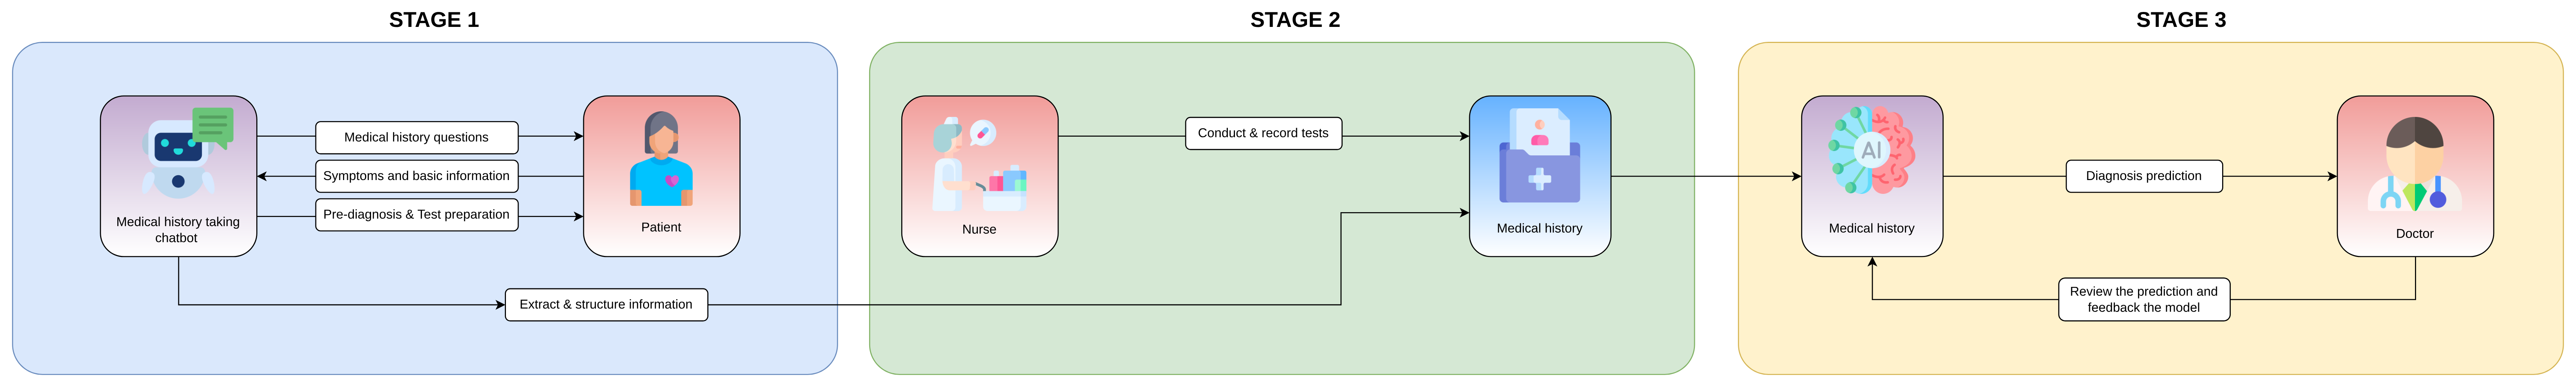
\includegraphics[width=\textwidth,height=0.7\textheight,keepaspectratio]{architecture.png}
\end{figure}

\begin{center}
\small Three stages from first contact to diagnosis, with a clinician in the loop at every step.
\end{center}

\end{frame}

%%%%%%%%%%%%%%%%%%%%%%%%%%%%%%%%%%%%%%%%%%%%%%%%%%%%%%%%%%%%%%%%%%%%%%%%%%%%%%%%%%%%%%%%%
\begin{frame}{The Three Stages}

\begin{columns}[t]
\column{0.3\textwidth}
\begin{block}{1\quad History taking}
\footnotesize\textit{Chatbot \& patient}
\begin{itemize}
	\item Chatbot asks medical history questions.
	\item Patient shares symptoms and basic information.
	\item Chatbot gives pre-diagnosis and test preparation.
	\item Answers are extracted and structured into the medical history.
\end{itemize}
\end{block}

\column{0.3\textwidth}
\begin{block}{2\quad Clinical testing}
\footnotesize\textit{Nurse}
\begin{itemize}
	\item Nurse conducts the tests the patient was prepared for.
	\item Results are recorded in the same structured medical history.
\end{itemize}
\end{block}

\column{0.3\textwidth}
\begin{block}{3\quad Diagnosis support}
\footnotesize\textit{AI model \& doctor}
\begin{itemize}
	\item Model predicts a diagnosis from the complete medical history.
	\item Doctor reviews the prediction.
	\item Doctor's feedback improves the model.
\end{itemize}
\end{block}
\end{columns}

\end{frame}

%%%%%%%%%%%%%%%%%%%%%%%%%%%%%%%%%%%%%%%%%%%%%%%%%%%%%%%%%%%%%%%%%%%%%%%%%%%%%%%%%%%%%%%%%
\section{Controllable History-Taking Agent}

\begin{frame}{Research Questions}
\framesubtitle{History-taking as a constrained POMDP: policy $\pi$, extractor $f$, quality $Q$}

\vspace{0.3cm}
\begin{columns}[T]
\column{0.46\textwidth}
\begin{block}{RQ1 -- Policy $\pi$}
\textbf{How should the agent choose its next action?}
\begin{itemize}
	\item Cover the PCOS guideline fields
	\item Follow the communication protocol
	\item Respect consent and safety
\end{itemize}
\end{block}
\column{0.46\textwidth}
\begin{block}{RQ2 -- Extractor $f$ and quality $Q$}
\textbf{How do we extract and assess a patient history?}
\begin{itemize}
	\item Facts, timing and chronology
	\item Evidence and uncertainty per field
	\item Coverage and factual accuracy
\end{itemize}
\end{block}
\end{columns}

\vspace{0.5cm}
\begin{center}
\small Initial use case: PCOS. Other conditions need their own schema and protocol.
\end{center}

\end{frame}

%%%%%%%%%%%%%%%%%%%%%%%%%%%%%%%%%%%%%%%%%%%%%%%%%%%%%%%%%%%%%%%%%%%%%%%%%%%%%%%%%%%%%%%%%
\begin{frame}{Proposed Agent Architecture}
\framesubtitle{The LLM handles language; state, policy and constraints stay explicit}

\begin{figure}
	\centering
	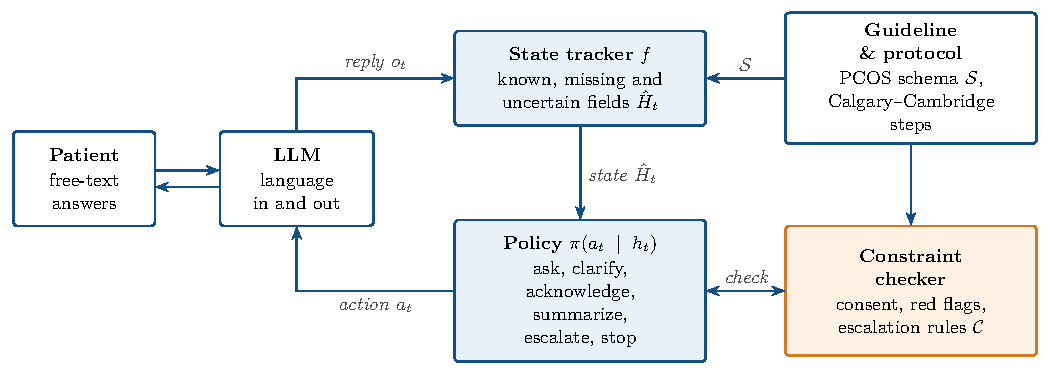
\includegraphics[width=0.95\textwidth,height=0.72\textheight,keepaspectratio]{agent-architecture.pdf}
\end{figure}

\end{frame}

%%%%%%%%%%%%%%%%%%%%%%%%%%%%%%%%%%%%%%%%%%%%%%%%%%%%%%%%%%%%%%%%%%%%%%%%%%%%%%%%%%%%%%%%%
\begin{frame}{Evaluation Plan}
\framesubtitle{Planned evaluation; no results are reported yet}

\vspace{0.2cm}
\begin{columns}[T]
\column{0.3\textwidth}
\begin{block}{Data and setting}
\small
\begin{itemize}
	\item MediTOD dialogues for extraction
	\item Simulated PCOS patients built from guideline profiles $z$
	\item Clinician-reviewed pilot cases
\end{itemize}
\end{block}
\column{0.3\textwidth}
\begin{block}{Metrics}
\small
\begin{itemize}
	\item \textbf{RQ2:} field coverage, accuracy, temporal consistency, unsupported claims
	\item \textbf{RQ1:} protocol adherence, turns $T$, correct escalation
\end{itemize}
\end{block}
\column{0.3\textwidth}
\begin{block}{Baselines}
\small
\begin{itemize}
	\item Prompt-only LLM
	\item Rule-based guideline checklist
	\item Hybrid: LLM with explicit policy and constraints
\end{itemize}
\end{block}
\end{columns}

\vspace{0.4cm}
\begin{center}
\small Reference standard: clinician-reviewed histories.
\end{center}

\end{frame}

%%%%%%%%%%%%%%%%%%%%%%%%%%%%%%%%%%%%%%%%%%%%%%%%%%%%%%%%%%%%%%%%%%%%%%%%%%%%%%%%%%%%%%%%%
\section{Status and Future Work}

\begin{frame}{Project Resources}

\setlstep{0.4cm}{0.1cm}{0cm}
\begin{itemize}
	\item \textbf{Video presentation} of the system: coming soon.
	\item \textbf{Interactive demo} of the chatbot: coming soon.
	\item \textbf{Project page}: \url{https://innovher-competition.github.io/demo/}
\end{itemize}

\end{frame}

%%%%%%%%%%%%%%%%%%%%%%%%%%%%%%%%%%%%%%%%%%%%%%%%%%%%%%%%%%%%%%%%%%%%%%%%%%%%%%%%%%%%%%%%%
\section{Conclusions}

\begin{frame}{Conclusions and Next Steps}

\begin{columns}[T]
\column{0.46\textwidth}
\begin{block}{Key messages}
\small
\setlstep{0.05cm}{0cm}{0cm}
\begin{itemize}
	\item For PCOS, the interview can inform two of three diagnostic criteria
	\item History-taking formulated as a constrained POMDP: policy $\pi$, extractor $f$, quality $Q$
	\item The proposed agent keeps state, policy and constraints explicit around the LLM
\end{itemize}
\end{block}
\column{0.46\textwidth}
\begin{block}{Next steps}
\small
\setlstep{0.05cm}{0cm}{0cm}
\begin{itemize}
	\item Build the PCOS schema $\mathcal{S}$ from the 2023 guideline
	\item Implement prompt-only, rule-based and hybrid policies
	\item Evaluate on MediTOD and simulated patients, then with clinician review
\end{itemize}
\end{block}
\end{columns}

\vspace{0.1cm}
\begin{alertblock}{Scope}
Clinician-reviewed history collection, not autonomous diagnosis.
\end{alertblock}

\end{frame}

%%%%%%%%%%%%%%%%%%%%%%%%%%%%%%%%%%%%%%%%%%%%%%%%%%%%%%%%%%%%%%%%%%%%%%%%%%%%%%%%%%%%%%%%%
\begin{frame}[plain,noframenumbering]
  \centering
  \vfill
  {\Huge\color{DEEblue} Thank you}\par
  \vspace{0.6cm}
  {\large Questions?}\par
  \vspace{1cm}
  {\small \url{https://innovher-competition.github.io/demo/}}\par
  \vspace{0.3cm}
  {\footnotesize huyen.le@etud.univ-evry.fr \quad thanhnamtran1605@gmail.com}
  \vfill
\end{frame}

%%%%%%%%%%%%%%%%%%%%%%%%%%%%%%%%%%%%%%%%%%%%%%%%%%%%%%%%%%%%%%%%%%%%%%%%%%%%%%%%%%%%%%%%%
% References: paste the paper's Reference.bib into this folder, cite with \cite{key},
% and uncomment the frame below.
%\section*{\bibname}
%\begin{frame}[t,allowframebreaks]
%	\makereferecesframe{Reference}
%\end{frame}

%%%%%%%%%%%%%%%%%%%%%%%%%%%%%%%%%%%%%%%%%%%%%%%%%%%%%%%%%%%%%%%%%%%%%%%%%%%%%%%%%%%%%%%%%
\end{document}
